
\documentclass[12pt]{article}
\usepackage[margin = 1in]{geometry}
\usepackage[dvipsnames]{xcolor}
\usepackage{tabularx}
\usepackage{graphicx}
\usepackage{enumitem}
\usepackage{hyperref}
% \usepackage{fancyhdr}
\usepackage[margin = 0cm]{caption}
\usepackage{wrapfig}
\usepackage{amsmath}
\usepackage{amssymb}
\usepackage{natbib}
\setlength{\bibsep}{0pt}
\hypersetup{ % all blue links
	colorlinks		= true,
	urlcolor 		= blue,
	linkcolor 		= blue,
	citecolor 		= blue
}
\setcitestyle{aysep={}, yysep={,}}
\newcommand{\aj}{AJ}
\newcommand{\aap}{A\&A}
\newcommand{\aapr}{A\&ARv}
\newcommand{\apj}{ApJ}
\newcommand{\apjl}{ApJL}
\newcommand{\apjs}{ApJS}
\newcommand{\apss}{Ap\&SS}
\newcommand{\araa}{ARA\&A}
\newcommand{\baas}{BAAS}
\newcommand{\fcp}{Fundamentals Cosmic Phys.}
\newcommand{\mnras}{MNRAS}
\newcommand{\nat}{Nature}
\newcommand{\pasa}{PASA}
\newcommand{\pasp}{PASP}
\newcommand{\ddfrac}[2]{\frac{\displaystyle{#1}}{\displaystyle{#2}}}
\newcommand{\msun}{\ensuremath{\text{M}_\odot}}
\newcommand{\scinote}[2]{\ensuremath{#1\times10^{#2}}}
\providecommand{\noopsort}[1]{}

\newcommand{\timescale}[1]{\ensuremath{\tau_\text{#1}}}
\newcommand{\harmonic}[2]{\ensuremath{\bar{\tau}_\text{[#1,#2]}}}
\newcommand{\hharmonic}[3]{\ensuremath{\bar{\tau}_\text{[#1,#2,#3]}}}
\renewcommand{\tilde}[1]{\ensuremath{\widetilde{#1}}}

\begin{document}

\begin{center}
\textbf{The Shape and Centroid of Abundance Distributions for Inside-Out Star
Formation Histories in One-Zone Models}
\par\null\par
James W. Johnson
\par\null\par
\rule[0.7\baselineskip]{0.5\textwidth}{0.4pt}
\end{center}

\par\noindent
\textbf{Analytic solution to~$Z_\alpha(t)$}
\par\noindent
The goal in this section is to obtain an analytic expression for the evolution
of the alpha element\footnote{
	As usual, an alpha element refers to, e.g., O or Mg. To be exact, it refers
	to an element whose only statistically significant enrichment source is a
	metallicity-independent population-averaged yield from massive stars.
} abundances~$Z_\alpha(t) \equiv M_\alpha / M_\text{g}$ using arguments similar
to those of~\citet*{Weinberg2017}.
For the purposes of these analytic approximations, I assume that the star
formation efficiency (SFE) timescale
$\tau_\star \equiv M_\text{g} / \dot{M}_\star$ and the outflow mass loading
factor~$\eta \equiv \dot{M}_\text{out} / \dot{M}_\star$ are both constant in
time.
Ultimately, this will be used to compute the metallicity distribution function
(MDF) according to
\begin{equation}
\frac{dN}{dZ_\alpha} = \frac{dN}{dt}/\frac{dZ_\alpha}{dt}
\propto \frac{\dot{M}_\star(t)}{\dot{Z}_\alpha(t)}.
\label{dndz}
\end{equation}
\par
For alpha elements,~\citet*{Weinberg2017} express the rate of change of the
mass present in the ISM as
\begin{equation}
\dot{M}_\alpha = y_\alpha \dot{M}_\star - Z_\alpha \dot{M}_\star (1 + \eta - r),
\label{eq:mdot_alpha}
\end{equation}
where~$r$ is a term which accounts for the return of stellar envelopes back to
the ISM.
Here I derive~$\dot{Z}_\alpha(t)$ assuming the ``inside-out'' star formation
history (SFH) from~\citet{Johnson2021}:
\begin{equation}
\dot{M}_\star(t) \propto (1 - e^{-t / \timescale{rise}})
e^{-t / \timescale{sfh}}.
\label{eq:insideout_sfh}
\end{equation}
The physically interesting advantage of this parameterization of the SFH over
the classic ``linear-times-exponential''~$t e^{-t / \timescale{sfh}}$ form is
that~$\timescale{rise}$ provides one with some control over how long the SFH is
increasing independent of~$\timescale{sfh}$.
\par
Based on the definition of~$Z_\alpha$, the quotient rule implies that its
time-derivative can be expressed as
\begin{subequations}\begin{align}
\dot{Z}_\alpha &= \frac{
	M_\text{g} \dot{M}_\alpha - M_\alpha \dot{M}_\text{g}
}{
	M_\text{g}^2
}
\\
&= \frac{
	M_\text{g} (y_\alpha \dot{M}_\star - Z_\alpha \dot{M}_\star (1 + \eta - r))
	- M_\alpha \ddot{M}_\star \tau_\star
}{
	M_\text{g}^2
}
\\
&= y_\alpha \frac{\dot{M}_\star}{M_\text{g}} -
Z_\alpha \frac{\dot{M}_\star}{M_\text{g}}(1 + \eta - r) -
Z_\alpha \frac{\ddot{M}_\star}{M_\text{g}} \tau_\star
\\
&= \frac{y_\alpha}{\tau_\star} -
Z_\alpha \left(\frac{1 + \eta - r}{\tau_\star} +
\frac{\ddot{M}_\star}{\dot{M}_\star}\right).
\label{eq:dzdt}
\end{align}\end{subequations}
The next step is to differentiate the SFH with time to compute
$\ddot{M}_\star / \dot{M}_\star$. Taking~$A$ to denote the overall normalizing
factor:
\begin{subequations}\begin{align}
\ddot{M}_\star &= \frac{d}{dt}
A(1 - e^{-t / \timescale{rise}}) e^{-t / \timescale{sfh}}
\\
&= A \frac{1}{\timescale{rise}}e^{-t / \timescale{rise}}
e^{-t / \timescale{sfh}} +
A(1 - e^{-t / \timescale{rise}}) \frac{-1}{\timescale{sfh}}
e^{-t / \timescale{sfh}}
\\
&= A(1 - e^{-t / \timescale{rise}})e^{-t / \timescale{sfh}}
\left(\frac{
	e^{-t / \timescale{rise}}
}{
	\timescale{rise}(1 - e^{-t / \timescale{rise}})
} - \frac{1}{\timescale{sfh}}
\right)
\\
\implies \frac{\ddot{M}_\star}{\dot{M}_\star} &= \frac{
	e^{-t / \timescale{rise}}
}{
	\timescale{rise}(1 - e^{-t / \timescale{rise}})
} - \frac{1}{\timescale{sfh}}.
\label{eq:mddotstar-over-mdotstar}
\end{align}\end{subequations}
At this point, it is straightforward to compute the equilibrium alpha element
abundance for this SFH by plugging equation~\ref{eq:mddotstar-over-mdotstar}
into equation~\ref{eq:dzdt} and setting~$\dot{Z}_\alpha = 0$.
This procedure results in the following expression:
\begin{equation}
Z_{\alpha,\text{eq}} = \ddfrac{
	y_\alpha
}{
	1 + \eta - r + \frac{
		e^{-t / \timescale{rise}}
	}{
		\timescale{rise}(1 - e^{-t / \timescale{rise}})
	} - \frac{\tau_\star}{\timescale{sfh}}
}.
\label{eq:zalpha-eq}
\end{equation}
Equation~\ref{eq:zalpha-eq} indicates that unlike the simpler SFHs like a
constant or single exponential, the equilibrium abundance is not uniform in
time.
Instead, the term depending on~\timescale{rise} is infinite at~$t = 0$,
increases at early times, and then approaches the solution for a single
exponential once~$t \gg \timescale{rise}$.
As a sanity check, equation~\ref{eq:zalpha-eq} indeed reduces to the
equilibrium abundance for a single exponential SFH found
by~\citet*{Weinberg2017} if I let~$\timescale{rise} \rightarrow 0$.
\par
Plugging this into equation~\ref{eq:dzdt} above yields the following linear
ODE for~$Z_\alpha$:
\begin{equation}
\dot{Z}_\alpha + Z_\alpha \left(\frac{1}{\timescale{dep}} +
\frac{
	e^{-t / \timescale{rise}}
}{
	\timescale{rise}(1 - e^{-t / \timescale{rise}})
} - \frac{1}{\timescale{sfh}}\right) = \frac{y_\alpha}{\tau_\star},
\end{equation}
where I have substituted for the depletion time, defined as
$\timescale{dep} \equiv \tau_\star / (1 + \eta - r)$.
$\timescale{dep}$ quantifies the e-folding timescale on which the ISM would
decline due to both star formation and mass loading, if present.
For notational convenience, I define the function~$f(t)$ to denote the
multiplicative factor on~$Z_\alpha$:
\begin{equation}
f(t) \equiv \frac{1}{\timescale{dep}} + \frac{
	e^{-t / \timescale{rise}}
}{
	\timescale{rise}(1 - e^{-t / \timescale{rise}})
} - \frac{1}{\timescale{sfh}},
\end{equation}
such that the general solution for~$Z_\alpha$ can be expressed as
\begin{equation}
Z_\alpha(t) = \exp\left(-\int f(t') dt'\right)\left(
\int_0^t \exp\left(\int f(t') dt'\right) \frac{y_\alpha}{\tau_\star} dt' + C
\right),
\label{eq:za-linear-ode}
\end{equation}
where the constant~$C$ will later be assigned such that the initial
condition~$Z_\alpha(t = 0) = 0$ is satisfied.
At this point, it is helpful to zoom in on the integral of~$f(t)$.
Its term depending on~$\timescale{rise}$ can be integrated with a series of
variable substitutions:
\begin{subequations}\begin{align}
\int \frac{
	e^{-t / \timescale{rise}}
}{
	\timescale{rise}(1 - e^{-t / \timescale{rise}})
} dt
&= \int \frac{e^{-u}}{1 - e^{-u}} du
\qquad \left(u = \frac{t}{\timescale{rise}};~~du = \frac{1}{\timescale{rise}}
dt\right)
\\
&= \int \frac{dv}{v} \qquad \left(v = 1 - e^{-u};~~dv = e^{-u} du\right)
\\
&= \ln v
\\
&= \ln (1 - e^{-u})
\\
&= \ln (1 - e^{-t / \timescale{rise}})
\\
\implies \int f(t) dt
&= \frac{t}{\timescale{dep}} + \ln (1 - e^{-t / \timescale{rise}}) -
\frac{t}{\timescale{sfh}}.
\end{align}\end{subequations}
Solving equation~\ref{eq:za-linear-ode} amounts to integrating the sum of a
handful of exponentials with prefactors that depend on~\timescale{rise},
\timescale{dep}, and~\timescale{sfh} in a non-trivial way.
The full derivation is attached, and the final solution is given by
\begin{equation}
\begin{split}
Z_\alpha(t) &= \frac{1}{1 - e^{-t / \timescale{rise}}}
\left(\frac{y_\alpha}{1 + \eta - r}\right)
\bigg[\frac{
	\timescale{sfh}
}{
	\timescale{sfh} - \timescale{dep}
} \left(
1 - \exp\left(-t\frac{
	\timescale{sfh} - \timescale{dep}
}{
	\timescale{sfh}\timescale{dep}
}\right)
\right) -
\\
&\qquad \frac{
	\timescale{sfh}\timescale{rise}
}{
	\timescale{sfh}\timescale{rise} - \timescale{dep}\timescale{rise} -
	\timescale{sfh}\timescale{dep}
} \left(e^{-t / \timescale{rise}} -
\exp\left(-t
\frac{
	\timescale{sfh} - \timescale{dep}
}{
	\timescale{sfh}\timescale{dep}
}
\right)
\right)\bigg].
\end{split}
\label{eq:zalpha}
\end{equation}
Adopting the harmonic timescale notation~$\harmonic{X}{Y} = \timescale{Y}
\timescale{X} / (\timescale{Y} - \timescale{X})$ of~\citet*{Weinberg2017}
simplifies the expression:
\begin{equation}
\begin{split}
Z_\alpha(t) &= \frac{1}{1 - e^{-t / \timescale{rise}}} \left( \frac{
	y_\alpha
}{
	1 + \eta - r
}\right) \bigg[
\frac{\harmonic{dep}{sfh}}{\timescale{dep}}
\left(1 - e^{-t / \harmonic{dep}{sfh}}\right) -
\\
&\qquad \frac{\hharmonic{dep}{rise}{sfh}}{\timescale{dep}}
\left(e^{-t / \timescale{rise}} - e^{-t / \harmonic{dep}{sfh}}\right)
\bigg]
\end{split}
\end{equation}
\par
At~$t = 0$, the factor~$1 / (1 - e^{-t / \timescale{rise}})$ is infinite,
but the factor enclosed in square brackets is zero.
Therefore, a physical solution exists if and only if the integration
constant~$C$, included in the full derivation of this expression (see equation
\ref{eq:zalpha-full}), is equal to zero.
Because this results in the~$\infty \times 0$ indeterminate form, I can simply
define the abundance to be zero such that the boundary condition
of~$Z_\alpha(t = 0) = 0$ is satisfied.

\begin{figure*}
\centering
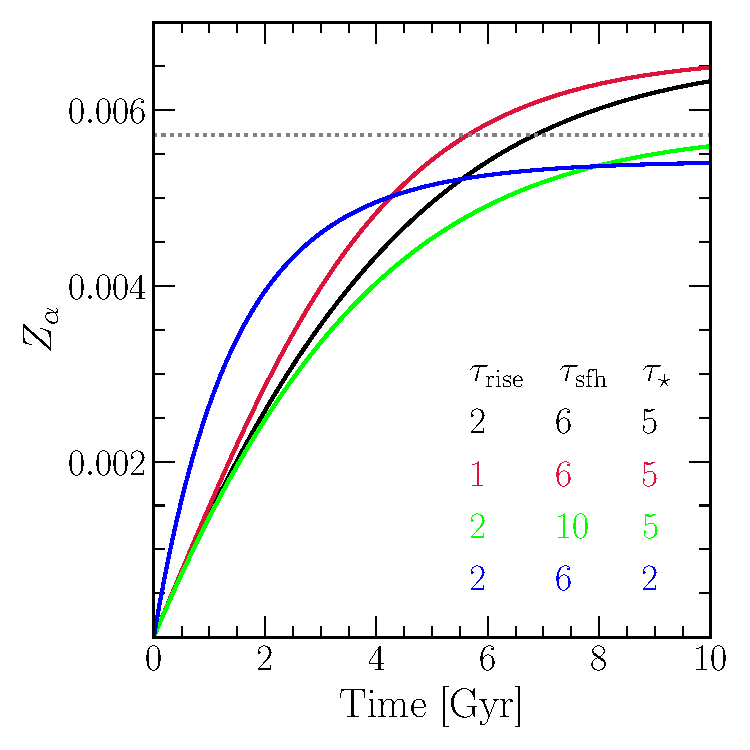
\includegraphics[scale = 0.52]{vartimescales.pdf}
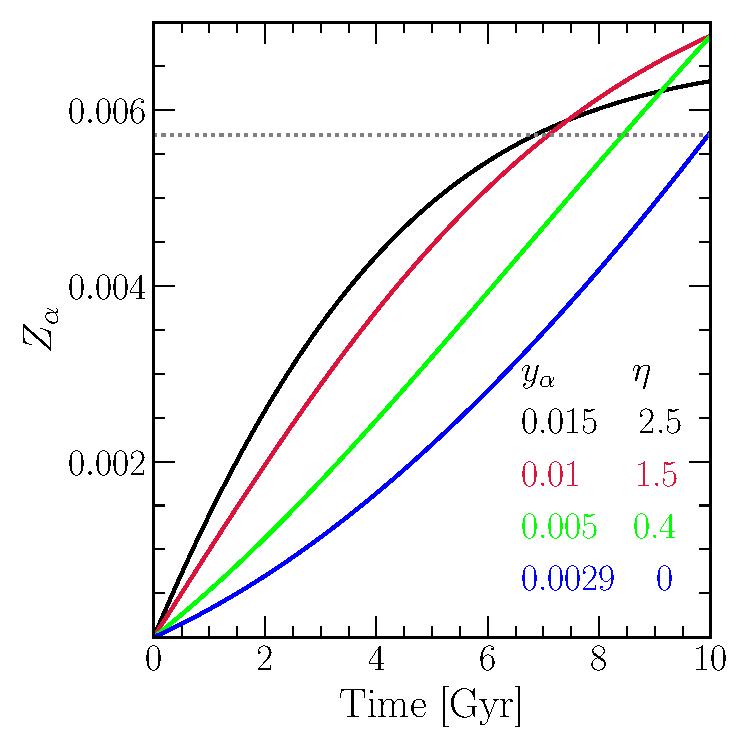
\includegraphics[scale = 0.52]{varyieldeta.pdf}
\caption{
Analytically computed evolution in the oxygen abundance according to equation
\ref{eq:zalpha}.
\textbf{Left}: For~$y_\alpha = 0.015$ and~$\eta = 2.5$, each curve denotes a
different choice of some timescale.
With black visualizing a fiducial choice of parameters of (\timescale{rise},
\timescale{sfh},~$\tau_\star$) = (2 Gyr, 6 Gyr, 5 Gyr), crimson shows a short
rise timescale (i.e.,~$\timescale{rise} = 1$ Gyr), lime green shows a more
extended SFH (i.e.,~$\timescale{sfh} = 10$ Gyr), and blue shows a higher SFE
(i.e.,~$\tau_\star = 2$ Gyr).
\textbf{Right}: For the fiducial choice of timescales in the right-hand panel,
each curve denotes a different choice of~$y_\alpha$ and~$\eta$ as denoted in
the legend.
For each choice of~$y_\alpha$, the value of~$\eta$ is chosen such that the
ratio~$y_\alpha / (1 + \eta - r)$ is approximately constant, and vice versa in
the case of the blue line where I choose~$\eta = 0$ and compute the
corresponding value of~$y_\alpha$.
}
\label{fig:analytic-evolution}
\end{figure*}

The left panel of Fig.~\ref{fig:analytic-evolution} visualizes the evolution of
the alpha element abundances according to equation~\ref{eq:zalpha} under
different choices of timescales.
% A shorter rise timescale has the effect of raising the abundances overall
\par
The right panel of Fig.~\ref{fig:analytic-evolution} visualizes the enrichment
history for the fiducial choice of timescales in the left panel, but with
different values of~$y_\alpha$ and~$\eta$, selected such that the value of
$y_\alpha / (1 + \eta - r)$ is approximately constant.

\newpage
\bibliographystyle{mnras}
\bibliography{onezone-mdfs}

\newpage
\noindent
\textbf{Full Solution to Equation~\ref{eq:za-linear-ode}}

\begin{subequations}\begin{align}
\begin{split} % a
Z_\alpha(t) &= \exp\left(
\frac{-t}{\timescale{dep}} - \ln (1 - e^{-t / \timescale{rise}}) +
\frac{t}{\timescale{sfh}}
\right)
\\
&\qquad \left[
\int_0^t \exp\left(
\frac{t'}{\timescale{dep}} + \ln (1 - e^{-t / \timescale{rise}}) -
\frac{t'}{\timescale{sfh}}
\right)
\frac{y_\alpha}{\tau_\star} dt' + C
\right]
\end{split}
\\
\begin{split} % b
&= \frac{1}{1 - e^{-t / \timescale{rise}}}
\exp \left(-t\frac{
	\timescale{sfh} - \timescale{dep}
}{
	\timescale{sfh}\timescale{dep}
}\right) \frac{y_\alpha}{\tau_\star}
\\
&\qquad \left[ \int_0^t (1 - e^{-t' / \timescale{rise}}) \exp \left(
t' \frac{\timescale{sfh} - \timescale{dep}}{\timescale{sfh} \timescale{dep}}
\right)dt' + C\right]
\end{split}
\\
\begin{split} % c
&= \frac{1}{1 - e^{-t / \timescale{rise}}}
\exp \left(-t\frac{
	\timescale{sfh} - \timescale{dep}
}{
	\timescale{sfh}\timescale{dep}
}\right) \frac{y_\alpha}{\tau_\star}
\\
&\qquad \left[ \int_0^t \left(
\exp\left(t' \frac{
	\timescale{sfh} - \timescale{dep}
}{
	\timescale{sfh}\timescale{dep}
}\right)
- \exp\left(
t' \frac{
	\timescale{sfh} - \timescale{dep}
}{
	\timescale{sfh}\timescale{dep}
} - \frac{t}{\timescale{rise}}
\right)
\right) dt' + C\right]
\end{split}
\\
\begin{split} % d
&= \frac{1}{1 - e^{-t / \timescale{rise}}}
\exp \left(-t\frac{
	\timescale{sfh} - \timescale{dep}
}{
	\timescale{sfh}\timescale{dep}
}\right) \frac{y_\alpha}{\tau_\star} \bigg[ \int_0^t
\exp\left(t'\frac{
	\timescale{sfh} - \timescale{dep}
}{
	\timescale{sfh}\timescale{dep}
} \right) dt' -
\\
&\qquad
\int_0^t \exp\left(t'\frac{
	\timescale{sfh}\timescale{rise} - \timescale{dep}\timescale{rise} -
	\timescale{sfh}\timescale{dep}
}{
	\timescale{sfh}\timescale{dep}\timescale{rise}
}\right) dt' + C \bigg]
\end{split}
\\
\begin{split} % e
&= \frac{1}{1 - e^{-t / \timescale{rise}}}
\exp \left(-t\frac{
	\timescale{sfh} - \timescale{dep}
}{
	\timescale{sfh}\timescale{dep}
}\right) \frac{y_\alpha}{\tau_\star} \bigg[\frac{
	\timescale{sfh}\timescale{dep}
}{
	\timescale{sfh} - \timescale{dep}
} \exp \left(t' \frac{
	\timescale{sfh} - \timescale{dep}
}{
	\timescale{sfh}\timescale{dep}
}\right) \bigg|_0^t -
\\
&\qquad \frac{
	\timescale{sfh}\timescale{dep}\timescale{rise}
}{
	\timescale{sfh}\timescale{rise} - \timescale{dep}\timescale{rise} -
	\timescale{sfh}\timescale{dep}
} \exp\left(
t'\frac{
	\timescale{sfh}\timescale{rise} - \timescale{dep}\timescale{rise} -
	\timescale{sfh}\timescale{dep}
}{
	\timescale{sfh}\timescale{dep}\timescale{rise}
}
\right)\bigg|_0^t + C \bigg]
\end{split}
\\
\begin{split} % f
&= \frac{1}{1 - e^{-t / \timescale{rise}}}
\exp \left(-t\frac{
	\timescale{sfh} - \timescale{dep}
}{
	\timescale{sfh}\timescale{dep}
}\right) \frac{y_\alpha}{\tau_\star} \bigg[\frac{
	\timescale{sfh}\timescale{dep}
}{
	\timescale{sfh} - \timescale{dep}
} \left(
\exp\left(
t\frac{
	\timescale{sfh} - \timescale{dep}
}{
	\timescale{sfh}\timescale{dep}
}\right) - 1\right) -
\\
&\qquad \frac{
	\timescale{sfh}\timescale{dep}\timescale{rise}
}{
	\timescale{sfh}\timescale{rise} - \timescale{dep}\timescale{rise} -
	\timescale{sfh}\timescale{dep}
} \left(
\exp\left(t\frac{
	\timescale{sfh}\timescale{rise} - \timescale{dep}\timescale{rise} -
	\timescale{sfh}\timescale{dep}
}{
	\timescale{sfh}\timescale{dep}\timescale{rise}
}\right) - 1\right)
\\
&\qquad + C\bigg]
\end{split}
\\
\begin{split} % g
&= \frac{1}{1 - e^{-t / \timescale{rise}}}
\left(\frac{y_\alpha}{\tau_\star}\right)
\bigg[\frac{
	\timescale{sfh}\timescale{dep}
}{
	\timescale{sfh} - \timescale{dep}
} \left(
1 - \exp\left(-t\frac{
	\timescale{sfh} - \timescale{dep}
}{
	\timescale{sfh}\timescale{dep}
}\right)
\right) -
\\
&\qquad \frac{
	\timescale{sfh}\timescale{dep}\timescale{rise}
}{
	\timescale{sfh}\timescale{rise} - \timescale{dep}\timescale{rise} -
	\timescale{sfh}\timescale{dep}
} \left(e^{-t / \timescale{rise}} -
\exp\left(-t
\frac{
	\timescale{sfh} - \timescale{dep}
}{
	\timescale{sfh}\timescale{dep}
}
\right)
\right) + C\bigg]
\end{split}
\\
\begin{split} % h
&= \frac{1}{1 - e^{-t / \timescale{rise}}}
\left(\frac{y_\alpha}{1 + \eta - r}\right)
\bigg[\frac{
	\timescale{sfh}
}{
	\timescale{sfh} - \timescale{dep}
} \left(
1 - \exp\left(-t\frac{
	\timescale{sfh} - \timescale{dep}
}{
	\timescale{sfh}\timescale{dep}
}\right)
\right) -
\\
&\qquad \frac{
	\timescale{sfh}\timescale{rise}
}{
	\timescale{sfh}\timescale{rise} - \timescale{dep}\timescale{rise} -
	\timescale{sfh}\timescale{dep}
} \left(e^{-t / \timescale{rise}} -
\exp\left(-t
\frac{
	\timescale{sfh} - \timescale{dep}
}{
	\timescale{sfh}\timescale{dep}
}
\right)
\right) + C\bigg].
\end{split}
\label{eq:zalpha-full}
\end{align}\end{subequations}

\newpage
\noindent
\textbf{Time-Derivative of~$Z_\alpha(t)$}
\par\noindent
Taking the time-derivative of equation~\ref{eq:zalpha} first and foremost
requires product rule.
It is helpful to split this process up into pieces:
\begin{subequations}\begin{align}
\frac{d}{dt} (1 - e^{-t / \timescale{rise}})^{-1} &=
-(1 - e^{-t / \timescale{rise}})^{-2}\frac{d}{dt}e^{-t / \timescale{rise}}
\\
&= \frac{
	e^{-t / \timescale{rise}}
}{
	\timescale{rise} (1 - e^{-t / \timescale{rise}})^2
}.
\end{align}\end{subequations}
To save space, I define the function~$g(t)$ to denote the term in square
brackets in equation~\ref{eq:zalpha}.
Its time derivative:
\begin{subequations}\begin{align}
\begin{split} % a
\dot{g}(t) &= \frac{\timescale{sfh}}{\timescale{sfh} - \timescale{dep}}
\exp \left( -t \frac{
	\timescale{sfh} - \timescale{dep}
}{
	\timescale{sfh}\timescale{dep}
}\right)\frac{
	\timescale{sfh} - \timescale{dep}
}{
	\timescale{sfh}\timescale{dep}
} - 
\\
&\qquad \frac{
	\timescale{sfh}\timescale{rise}
}{
	\timescale{sfh}\timescale{rise} - \timescale{dep}\timescale{rise} -
	\timescale{sfh}\timescale{dep}
} \bigg(
\frac{-1}{\timescale{rise}} e^{-t / \timescale{rise}} +
\\
&\qquad
\exp \left( -t \frac{
	\timescale{sfh} - \timescale{dep}
}{
	\timescale{sfh}\timescale{dep}
}
\right)
\frac{
	\timescale{sfh} - \timescale{dep}
}{
	\timescale{sfh}\timescale{dep}
}
\bigg)
\end{split}
\\
\begin{split} % b
&= \frac{1}{\timescale{dep}}\exp\left( -t \frac{
	\timescale{sfh} - \timescale{dep}
}{
	\timescale{sfh}\timescale{dep}
}\right) + \frac{
	\timescale{sfh}
}{
	\timescale{sfh}\timescale{rise} - \timescale{dep}\timescale{rise} -
	\timescale{sfh}\timescale{dep}
} e^{-t / \timescale{rise}} -
\\
&\qquad \frac{
	\timescale{rise}\timescale{sfh} - \timescale{rise}\timescale{dep}
}{
	\timescale{sfh}\timescale{rise}\timescale{dep} - \timescale{dep}^2
	\timescale{rise} - \timescale{sfh}\timescale{dep}^2
} \exp \left( -t \frac{
	\timescale{sfh} - \timescale{dep}
}{
	\timescale{sfh}\timescale{dep}
}
\right)
\end{split}
\\
\begin{split} % c
&= \exp\left(-t \frac{
	\timescale{sfh} - \timescale{dep}
}{
	\timescale{sfh}\timescale{dep}
}\right) \bigg[
\frac{1}{\timescale{dep}} - \frac{
	\timescale{rise}\timescale{sfh} - \timescale{rise}\timescale{dep}
}{
	\timescale{sfh}\timescale{rise}\timescale{dep} - \timescale{dep}^2
	\timescale{rise} - \timescale{sfh}\timescale{dep}^2
} +
\\
&\qquad \frac{
	\timescale{sfh}
}{
	\timescale{sfh}\timescale{rise} - \timescale{dep}\timescale{rise} -
	\timescale{sfh}\timescale{dep}
} \exp \left(t \frac{
	\timescale{rise}\timescale{sfh} - \timescale{dep}\timescale{rise} -
	\timescale{sfh}\timescale{dep}
}{
	\timescale{rise}\timescale{sfh}\timescale{dep}
}\right) \bigg]
\end{split}
\\
\begin{split} % d
&= \exp\left(-t \frac{
	\timescale{sfh} - \timescale{dep}
}{
	\timescale{sfh}\timescale{dep}
}\right) \frac{
	\timescale{sfh}
}{
	\timescale{sfh}\timescale{rise} - \timescale{dep}\timescale{rise} -
	\timescale{sfh}\timescale{dep}
}
\\
&\qquad \left[\exp\left(t \frac{
	\timescale{rise}\timescale{sfh} - \timescale{dep}\timescale{rise} -
	\timescale{sfh}\timescale{dep}
}{
	\timescale{rise}\timescale{sfh}\timescale{dep}
}\right)
- 1\right].
\end{split}
\end{align}\end{subequations}
At this point, it simplifies notation to define
\begin{equation}
\hharmonic{dep}{sfh}{rise} \equiv \frac{
	\timescale{rise}\timescale{sfh}\timescale{dep}
}{
	\timescale{sfh}\timescale{rise} - \timescale{dep}\timescale{rise} -
	\timescale{sfh}\timescale{dep}
} = \left( \frac{1}{\timescale{dep}} - \frac{1}{\timescale{sfh}} -
\frac{1}{\timescale{rise}}\right)^{-1},
\end{equation}
which is reminiscent of the harmonic timescales~$\harmonic{X}{Y}$ seen
in~\citet*{Weinberg2017}, but for three timescales instead of two.
Adopting this notation yields the following expression for~$\dot{g}(t)$:
\begin{equation}
\begin{split}
\dot{g}(t) &= \frac{
	\hharmonic{dep}{rise}{sfh}
}{
	\timescale{rise}\timescale{dep}
} e^{-t / \harmonic{dep}{sfh}} \left(e^{t /
\hharmonic{dep}{rise}{sfh}} - 1\right)
\\
&= \frac{
	\hharmonic{dep}{rise}{sfh}
}{
	\timescale{rise}\timescale{dep}
} \left(e^{-t / \timescale{rise}} - e^{-t / \harmonic{dep}{sfh}}\right).
\end{split}
\end{equation}
I can now write the full expression for~$\dot{Z}_\alpha(t)$:
\begin{subequations}\begin{align}
\dot{Z}_\alpha(t) &= \left(\frac{y_\alpha}{1 + \eta - r}\right)
\left[
\frac{e^{-t / \timescale{rise}}}{
	\timescale{rise} (1 - e^{-t / \timescale{rise}})^2
} g(t) + \frac{1}{1 - e^{-t / \timescale{rise}}} \dot{g}(t)
\right]
\\
&= \left(\frac{y_\alpha}{1 + \eta - r}\right)
\frac{1}{1 - e^{-t / \timescale{rise}}} \left[
\dot{g}(t) + \frac{
	e^{-t / \timescale{rise}}
}{
	\timescale{rise} (1 - e^{-t / \timescale{rise}})
} g(t)
\right],
\end{align}\end{subequations}
and an expression for~$\dot{Z}_\alpha(t) / Z_\alpha(t)$:
\begin{subequations}\begin{align}
\frac{\dot{Z}_\alpha(t)}{Z_\alpha(t)} &= \ddfrac{
	\dot{g}(t) + \frac{
		e^{-t / \timescale{rise}}
	}{
		\timescale{rise} (1 - e^{-t / \timescale{rise}})
	} g(t)
}{
	g(t)
}
\\
&= \frac{\dot{g}(t)}{g(t)} + \frac{
	e^{-t / \timescale{rise}}
}{
	\timescale{rise} (1 - e^{-t / \timescale{rise}})
}.
\end{align}\end{subequations}
Expanding on $\dot{g}(t) / g(t)$:
\begin{subequations}\begin{align}
\frac{\dot{g}(t)}{g(t)} &= \left(\frac{g(t)}{\dot{g}(t)}\right)^{-1}
\\
&= \left[\ddfrac{
	\frac{
		\harmonic{dep}{sfh}
	}{
		\timescale{dep}
	} \left(1 - e^{-t / \harmonic{dep}{sfh}}\right) -
	\frac{
		\hharmonic{dep}{rise}{sfh}
	}{
		\timescale{dep}
	} \left(e^{-t / \timescale{rise}} -
	e^{-t / \harmonic{dep}{sfh}}\right)
}{
	\frac{
		\hharmonic{dep}{rise}{sfh}
	}{
		\timescale{rise}\timescale{dep}
	}
	\left(e^{-t / \timescale{rise}} - e^{-t / \harmonic{dep}{sfh}}
	\right)
}\right]^{-1}
\\
&= \frac{1}{\timescale{rise}}\left[1 -
\frac{
	\harmonic{dep}{sfh}
}{
	\hharmonic{dep}{rise}{sfh}
}\left(
\frac{
	1 - e^{-t / \harmonic{dep}{sfh}}
}{
	e^{-t / \timescale{rise} - e^{-t / \harmonic{dep}{sfh}}}
}
\right)
\right]^{-1},
\end{align}\end{subequations}
and therefore the final expression for~$\dot{Z}_\alpha(t) / Z_\alpha(t)$:
\begin{equation}
\frac{\dot{Z}_\alpha(t)}{Z_\alpha(t)} = \frac{
	e^{-t / \timescale{rise}}
}{
	\timescale{rise} (1 - e^{-t / \timescale{rise}})
} + \frac{1}{\timescale{rise}} \left[
1 - \frac{
	\harmonic{dep}{sfh}
}{
	\hharmonic{dep}{rise}{sfh}
}\left(\frac{
	1 - e^{-t / \harmonic{dep}{sfh}}
}{
	e^{-t / \timescale{rise} - e^{-t / \harmonic{dep}{sfh}}}
}\right)
\right]^{-1}
\end{equation}

\end{document}


























































